



\BiChapter{注释(需要删除)}{uuu}
%\caption{u}



%
%
%最近,光场显著性物体检测(LFSOD)因在复杂场景中利用丰富的光场线索取得显著改进而引起了越来越多的关注。虽然许多工作在这一领域取得了显著进展,但对其焦点特性的更深入洞察应该被开发。在这项工作中,我们提出了焦点感知变换器(FPT),可以高效地编码焦点堆栈内和全部焦点图像中的上下文。具体而言,我们引入了与焦点相关的令牌来总结图像特定特征,并且提出了令牌通信模块(TCM)来传达信息并促进空间上下文建模。通过精确编码的与焦点相关的令牌之间的信息交换,可以丰富每幅图像的特征并与其他图像相关联。我们还提出了焦点感知增强(FPE)策略,以帮助抑制嘈杂的背景信息。对四个广泛使用的基准数据集进行的大量实验证明,所提出的模型优于当前最先进的方法。我们的代码将公开提供。




% 
% 
% 
% 
% <<<<<<< HEAD
% 其中$m$索引注意力头,$k$索引采样键,
% $K$是采样键的总数($K \ll HW$),
% $\bigtriangleup p_{mqk} $和$A_{mqk}$分别表示
% 第$m^{th}$个注意力头中第$k^{th}$个采样点的采样偏移量和注意力权重。
% 标量注意力权重$A_{mqk}$位于$\left [ 0,~1 \right ] $范围内,
% 通过$ {\textstyle \sum_{k=1}^{K}} A_{mqk}=1$进行归一化。
% $\bigtriangleup p_{mqk} \in \mathbb{R}^{2}$
% 是范围不受约束的二维实数。
% 由于$p_{q} + \bigtriangleup p_{mqk}$是分数,如等人所述,
% $x\left ( p_{q} + \bigtriangleup p_{mqk} \right ) $在计算时应用双线性插值。
% $\bigtriangleup p_{mqk}   $和$A_{mqk}$都是通过查询特征$z_{q}$上的线性投影获得的。
% 在具体实现中,查询特征$z_{q}$被馈送到$3MK$通道的线性投影算子,
% 其中前$2MK$通道对采样偏移量$\bigtriangleup p_{mqk}$进行编码,
% 其余$MK$通道通过被馈送到$softmax$算子以获得注意力权重$A_{mqk}$。






% 可变形注意力模块旨在将卷积特征图作为关键元素进行处理。

% 设 为查询元素的数量,当较小时,可变形注意力模块的复杂度为。
% 当应用于DETR编码器时,其中,复杂度变为,
% 起复杂度与空间大小呈线性关系。
% 当它作为DETR解码器中的交叉注意力模块应用时,
% 其中,是对象查询的数量,复杂度变为,
% 这与空间大小无关。


% 多尺度可变形注意力模型。
% 大多数现代目标检测框架都受益于多尺度特征图。
% 我们提出的可变形注意力模块可以自然地扩展到多尺度特征图。
% 令为输入多尺度特征图,
% 其中。
% 令为每个查询元素的参考点的归一化坐标,
% 然后应用多尺度可变形注意力采样点。
% 分别表示第几个特征层和第几个注意力头中第几个采样点的采样偏移和注意力权重。
% 标量注意力权重通过进行归一化。

% 这里,为了尺度公式的清晰性,我们使用归一化坐标,
% 其中归一化坐标分别表示图像的左上角和右下角。
% 方程中的函数将归一化坐标重新放缩到第几层的输入特征图。


% 多尺度可变形注意力与之前的单尺度版本非常相似,只是它从多尺度特征图中采样点,
% 而不是从单尺度特征图中采样k个点。
% 当且固定为单位矩阵时,所提出的注意力模块将退化为可变形卷积。
% 可变形卷积是针对单尺度输入而设计的,每个注意力头仅关注一个采样点。
% 然而,我们的多尺度可变形注意力会关注来自多尺度输入的多个采样点。
% 所提出的(多尺度)可变形注意模块也可以被视为
% Transformer 注意的有效变体,其中通过可变形采样位置引入预过滤机制。
% 当采样点遍历所有可能得位置时,所提出的注意力模块相当于Transformer注意力。


% 可变形Transformer 编码器。

% 我们将网络中处理特征图的Transformer注意模块替换为所提出的多尺度可变形注意模块。
% 编码器的输入和输出都是具有相同分辨率的多尺度特征图。

% 在编码器中,我们从骨干网络中提取多尺度特征图,通过卷积,
% 其中的分辨率比输入图像低。
% 最低分辨率特征图是通过最后阶段的步长卷积获得的。

% 所有多尺度特征图均为个通道,
% 像FPN网络结构中,没有使用自上而下的结构,因为我们提出的多尺度可变形注意力本身可以在多尺度特征图之间交换信息。




%%
%%
%\begin{table*}[]
%	%
%	%---------------------------------------------------------------------> 大表 
%	%
%	%	\caption{Quantitative comparison of our proposed FPT with other 20 SOTA SOD methods on three benchmark datasets. 
%		%		$ \uparrow \& \downarrow $ denote larger and smaller is better.
%		%		%
%		%		% denote the best and the second-best results,
%		%		%
%		%		The best three results are shown in 
%		%		\textbf{boldface}, \textcolor{red}{red} and \textcolor{blue}{blue} fonts respectively. 
%		%		% '-' indicates the code or outcome is not available.
%		%	}
%	\bicaption{
%		在 3 个公开数据集上的定量比较
%	}{Quantitative comparisons on three light field datasets}
%	%	\renewcommand{\arraystretch}{1.5}
%	
%	\centering
%	\label{table:comp_with_sota_3_1}
%	%	\label{table:comp-with-sota}
%	\resizebox{\textwidth}{!}{
%		\begin{tabular}{rcccccccccccc}
%			\toprule  %添加表格头部粗线
%			
%			% title
%			%			\multirow{2}*{Type} & 
%			\multicolumn{1}{c}{ \multirow{2}*{方法} } & 
%			\multicolumn{4}{c}{DUTLF-FS \cite{zhang2019memory} } &
%			\multicolumn{4}{c}{HFUT \cite{zhang2017saliency} } &
%			\multicolumn{4}{c}{LFSD \cite{li2014saliency} } \\
%			
%			% next line
%			\cmidrule(r){2-5} \cmidrule(r){6-9} \cmidrule(r){10-13}
%			
%			%			 subtitle
%			& $E_{\phi}^{max}\uparrow$ & $S_{\alpha }\uparrow$ & $F_{\beta}^{max}\uparrow$ & MAE$\downarrow$ 
%			& $E_{\phi}^{max}\uparrow$ & $S_{\alpha }\uparrow$ & $F_{\beta}^{max}\uparrow$ & MAE$\downarrow$  
%			& $E_{\phi}^{max}\uparrow$ & $S_{\alpha }\uparrow$ & $F_{\beta}^{max}\uparrow$ & MAE$\downarrow$ \\
%			
%			%			& E & S & F & MAE 
%			%			& E & S & F & MAE 
%			%			& E & S & F & MAE \\
%			
%			
%			% line line
%			\midrule
%			
%			%			\multirow{8}*{\textit{Light field}}
%			
%			% 开始填数据
%			
%			Ours	 
%			&  {\textbf{.973}} & \textbf{ {.946}} 	& \textbf{ {.954}} & \textbf{ {.020}} 
%			& \textbf{ {.871}} &	\textbf{ {.828}} 			&\textbf{	 {.784}} & {\textcolor{red}{.064}} 
%			& \textbf{ {.919}} &	\textcolor{blue}{.860} 			&	\textbf{ {.873}} &	\textbf{ {.064}} 
%			\\
%			
%			DLGLRG \cite{liu2021light} 
%			& {\textcolor{red}{.958}} & {\textcolor{red}{.928}} 			& {\textcolor{red}{.934}} & {\textcolor{red}{.029}} 
%			&	.839 &	.766 &	.698 &	.070 
%			&	{\textcolor{red}{.906}} &	\textbf{ {.866}} 			&	{\textcolor{red}{.870}} &	\textcolor{blue}{.069} 
%			\\
%			
%			ERNet \cite{piao2020exploit}
%			& .947 & .899 & .908 & .039 
%			&	.841 &	.778 &	.722 &	.082 
%			&	.888 &	.834 &	.850 &	.082 
%			\\
%			
%			PANet \cite{piao2021panet} 
%			& .939 & .908 & .903 & .038 
%			& .845 & .795 & .738 & .074 
%			& .892 & .849 & .849 & .076
%			\\
%			
%			LFNet	 \cite{zhang2020lfnet} 
%			& .929 & .878 & .890 & .053
%			&	.846 &	.782 &	.718 &	.073 
%			&	.885 &	.820 &	.824 &	.092 \\
%			
%			MAC	 \cite{zhang2020light} 
%			& .863	& .804	& .792	& .102	
%			&   .797 & .731 & .667 & .107 
%			& .832 & .782 & .776 & .127 \\
%			
%			MoLF	 \cite{zhang2019memory} 
%			& .938 & .887 & .902 & .051 
%			&	.852 &	.789 &	.729 &	.075 
%			&	.888 &	.830 &	.834 &	.089 \\
%			
%			DLSD	\cite{piao2019deep}
%			& .891	& .841	& .801	& .076	
%			&   .783 & .741 & .615 & .098 
%			& .806 & .737 & .715 & .147 \\
%			
%			\midrule % end lfsod
%			
%			% start rgb-d
%			%			\multirow{6}*{\textit{RGB-D}}
%			
%			DCF \cite{ji2021calibrated} 
%			& \textcolor{blue}{.954} & \textcolor{blue}{.921} & \textcolor{blue}{.927} & \textcolor{blue}{.031} 
%			& \textcolor{blue}{.856} & {\textcolor{red}{.812}} & {\textcolor{red}{.768}} & \textcolor{blue}{.065} 
%			& .881 & .809 & .821 & .096 \\
%			
%			CIR-Net \cite{cong2022cir}
%			& .950 & .916 & .921 & .038 
%			& {\textcolor{red}{.862}} & .800  			& .742 & \textbf{ {.062}} 
%			& .874 & .820 & .816 & .098 \\ 
%			
%			VST-$rgbd$  \cite{liu2021visual} 
%			& .952 & .920 & .921 & .036 
%			& .843 & .807 & .754 & .086 
%			& .851 & .792 & .786 & .110 
%			\\
%			
%			%			& -  & 2022  & \\
%			%			& -  & 2022  & \\
%			
%			BBS-Net     \cite{fan2020bbs} 
%			& .900 & .865 & .852 & .066 
%			& .801 & .751 & .676 & .073 
%			& \textcolor{blue}{.901} & {\textcolor{red}{.864}} & .858 & .072 \\ 
%			
%			SSF     \cite{zhang2020select} 
%			& .922 & .879 & .887 & .050 
%			& .816 & .725 & .647 & .090 
%			& \textcolor{blue}{.901} & .859 & \textcolor{blue}{.868} & {\textcolor{red}{.067}} \\ 
%			
%			S2MA    \cite{liu2020learning} 
%			& .839 & .787 & .754 & 	.102 
%			& .777 & .729 & .650 & .112 
%			& .873 & .837 &	.835 & .094 \\
%			
%			
%			\midrule % end rgb-d
%			%			\multirow{7}*{\textit{RGB}}
%			
%			VST-$rgb$ \cite{liu2021visual} 
%			& .939 & .910 & .911 & .047
%			& .831 & \textcolor{blue}{.808} & \textcolor{blue}{.763} & .093 
%			& .865 & .797 & .817 & .123 
%			\\ 
%			
%			PFSNet \cite{ma2021pyramidal}
%			& .912 & .883 & .879 & .057 
%			& .835 & .800 & .752 & .088 
%			& .805 & .749 & .727 & .145 
%			\\ 
%			
%			
%			ITSD \cite{zhou2020interactive} 
%			& .930 & .899 & .899 & .052 
%			& .839 & .805 & .759 & .089 
%			& .879 & .847 & .840 & .088 
%			\\ 
%			
%			
%			
%			LDF \cite{wei2020label} 
%			& .898 & .873 & .861 & .061 
%			& .804 & .780 & .708 & .093 
%			& .843 & .821 & .803 & .096 
%			\\ 
%			
%			
%			MINet \cite{pang2020multi} 
%			& .916 & .890 & .882 & .050 
%			& .816 & .792 & .720 & .086 
%			& .861 & .834 & .828 & .091 
%			\\ 
%			
%			F$^{3}$Net  \cite{wei2020f3net}
%			& .900 & .888 & .882 & .057 
%			& .815 & .777 & .718 & .095 
%			& .824 & .806 & .797 & .106 
%			\\ 
%			
%			
%			EGNet   \cite{zhao2019egnet}
%			& .914 & .886 & .870 & .053 
%			& .794 & .772 & .672 & .094 
%			& .776 & .784 & .762 & .118 
%			\\ 
%			
%			CPD  \cite{wu2019cascaded}
%			& .867 & .911 & .866 & .058 
%			& .772 & .82  & .701 & .086 
%			& .759 & .82  & .759 & .126 \\
%			
%			PoolNet \cite{liu2019simple}
%			& .889 & .919 & .868 & .051 
%			& .776 & .802 & .683 & .092 
%			& .789 & .8   & .769 & .118 \\
%			
%			PiCANet \cite{liu2018picanet}
%			& .829 & .892 & .821 & .083 
%			& .726 & .781 & .618 & .115 
%			& .729 & .78  & .671 & .158 \\
%			
%			PAGRN \cite{wang2018detect}
%			& .822 & .878 & .828 & .084 
%			& .717 & .773 & .635 & .114 
%			& .727 & .805 & .725 & .147 \\
%			
%			C2S   \cite{li2018contour}
%			& .844 & .874 & .791 & .084 
%			& .763 & .786 & .65  & .111 
%			& .806 & .82  & .749 & .113 \\
%			
%			R3Net  \cite{deng2018r3net}
%			& .833 & .819 & .783 & .113 
%			& .727 & .728 & .625 & .151 
%			& .789 & .838 & .781 & .128 \\
%			
%			Amulet \cite{zhang2017amulet}
%			& .847 & .882 & .805 & .030 
%			& .767 & .76  & .636 & .110  
%			& .773 & .821 & .757 & .135 \\
%			
%			
%			\bottomrule % end
%		\end{tabular}
%	}
%\end{table*}
%%
%%
%%\\
%%\\


































%
%%
%%
%%\par
%\begin{figure}[!ht]
%	\centering
%	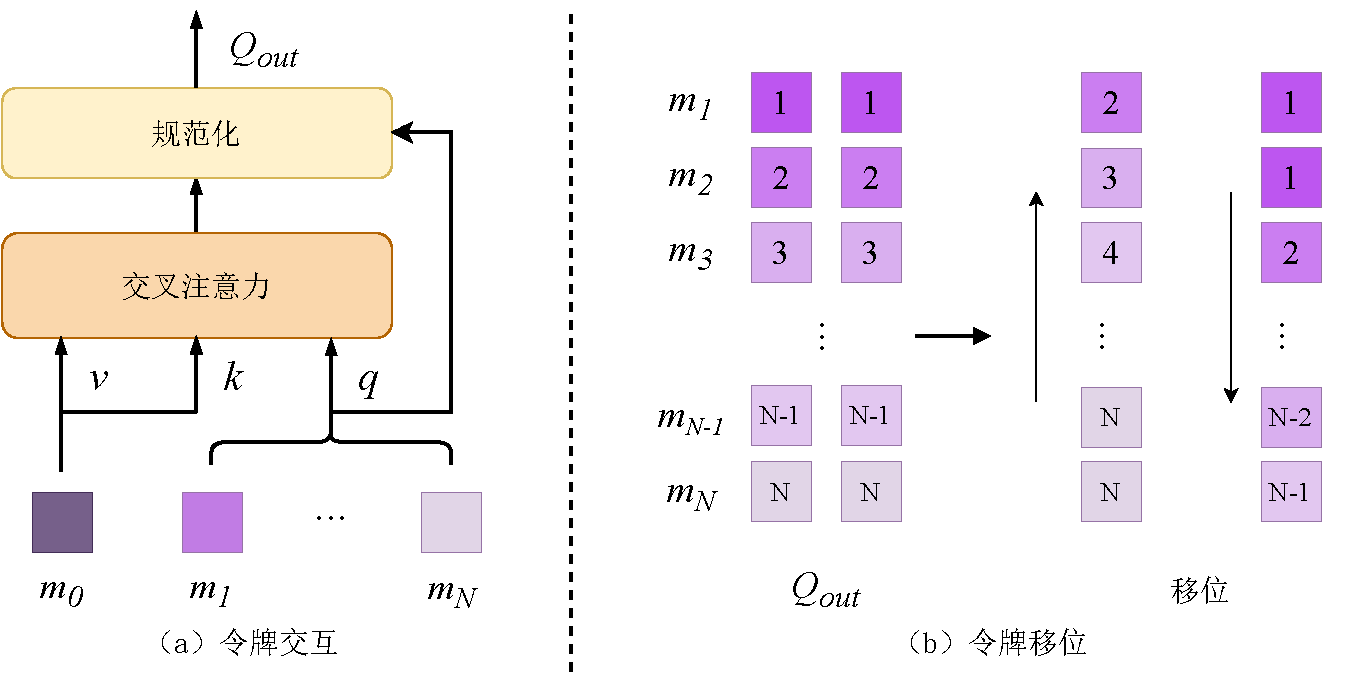
\includegraphics[width=0.95\linewidth]{figures/chapter3/token-interaction.drawio}
%	\bicaption{
%		令牌通信模块 (TCM) 的图示。
%		(a) 令牌交互(TI)。 
%		(b) 令牌移位(TS)。 
%	}{
%		An illustration of the Token Communication Module (TCM). 
%		(a) Token Interaction (TI). 
%		(b) Token Shift (TS).
%	}  
%	\label{cpt3_fig1:token_interaction}
%\end{figure}
%%
%%
















%
%
%%
%%---------------------------------------------------------------------> fig: 创新图
%\begin{figure}[!ht]
%	\centering
%	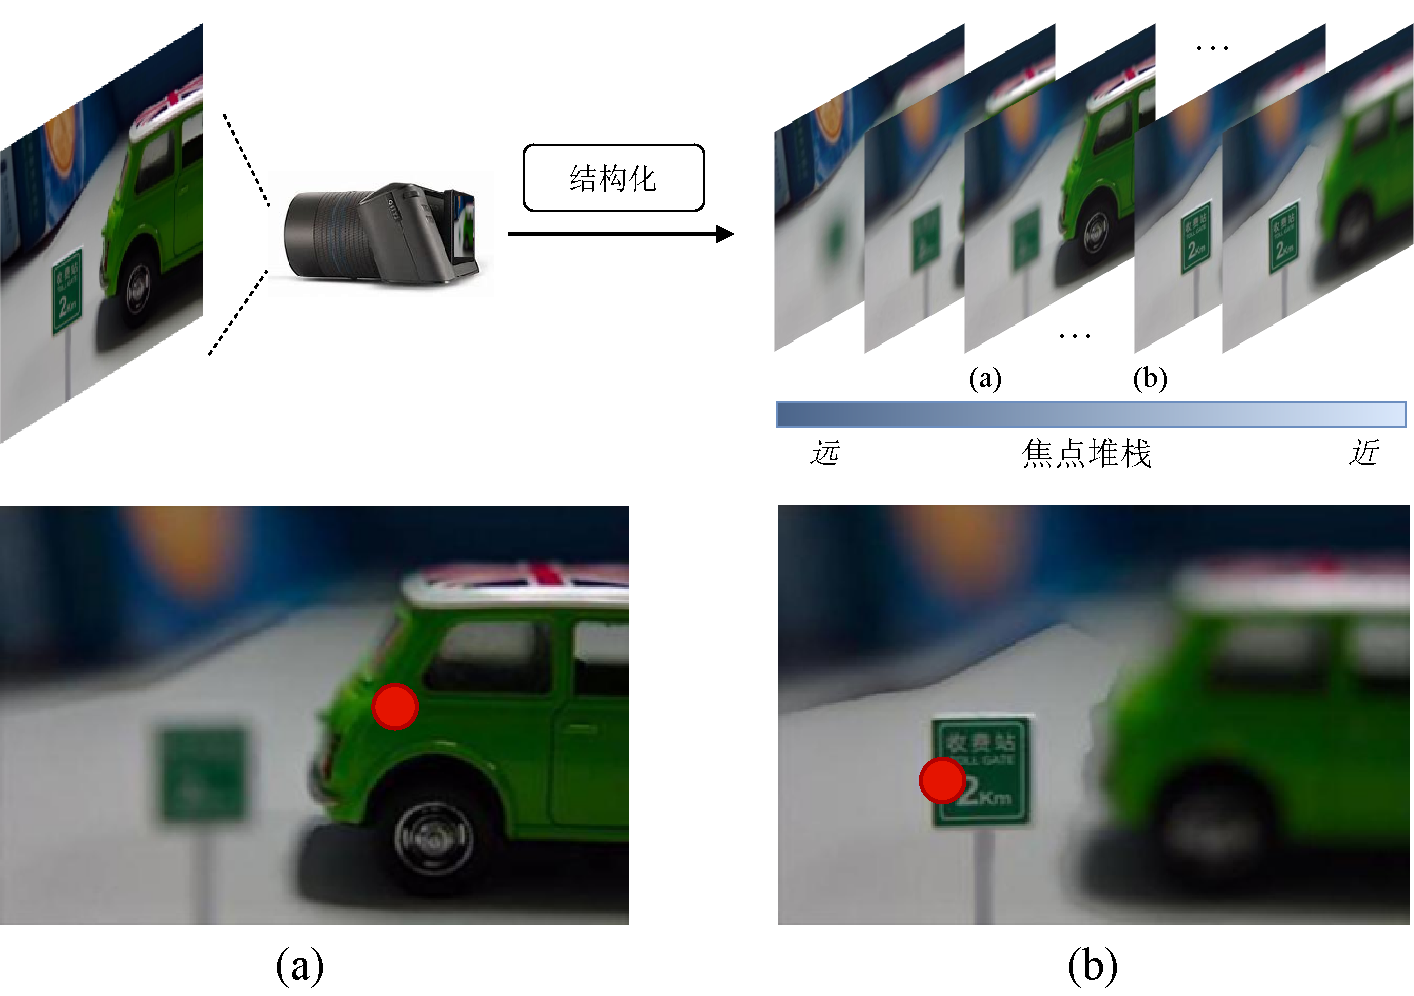
\includegraphics[width=0.85\linewidth]{figures/chapter3/cpt3_idea.pdf}
%	\bicaption{
%		光场焦点堆栈的成像过程和不同切片的成像效果。
%		\textcolor{red}{$\bullet$} 表示清晰的部分。
%	}
%	{ 
%		The imaging process of the light field focus stack and the imaging effects of different slices.
%		\textcolor{red}{$\bullet$} indicates the clear parts.  
%	}
%	\label{figure:cpt3:idea}
%\end{figure}
%%
%%


















%
%%------------------------------ figure: comparison
%\begin{figure}[!ht]
%	\centering
%	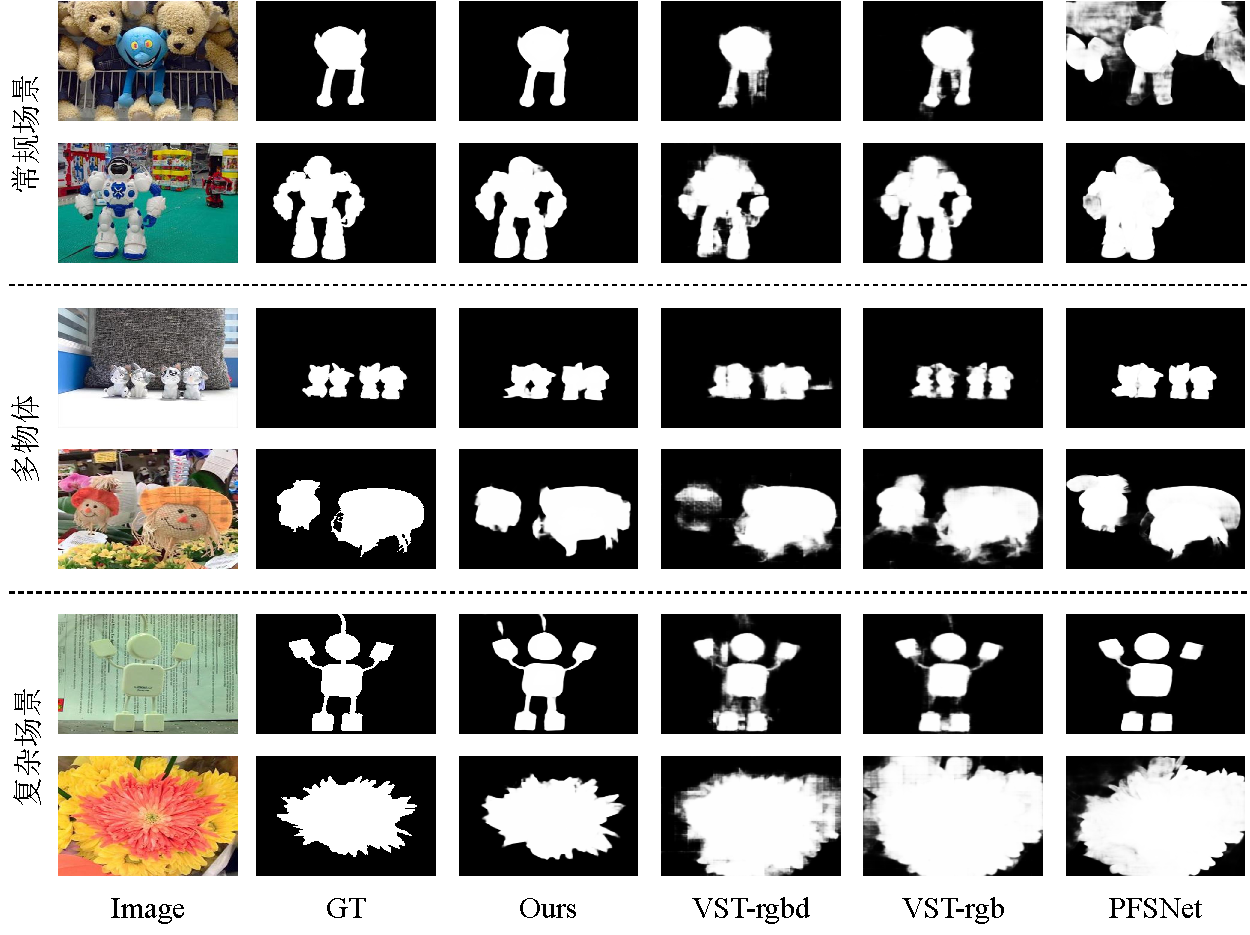
\includegraphics[width=\linewidth]{figures/chapter3/compare_3}
%	%	\caption{
%		%		Qualitative comparisons of state-of-the-art methods in some challenging scenes, including multiple objects and complex scenes.
%		%	}
%	\bicaption{
%		在一些具有挑战性的场景(包括多物体和复杂场景)中对最先进的方法进行定性比较。
%	}{
%		Qualitative comparisons of state-of-the-art methods in some challenging scenes, including multiple objects and complex scenes.
%	}
%	\label{chpt4:fig:comparison_3}
%	\vspace{-0.2cm}
%\end{figure}
%% 
%%
%










%
%\begin{figure}[!ht] 
%	% \centering
%	%	\begin{center}
%		%	\includegraphics[width=0.95\linewidth]{figures/overview.pdf} 		
%		%	\end{center}
%	
%	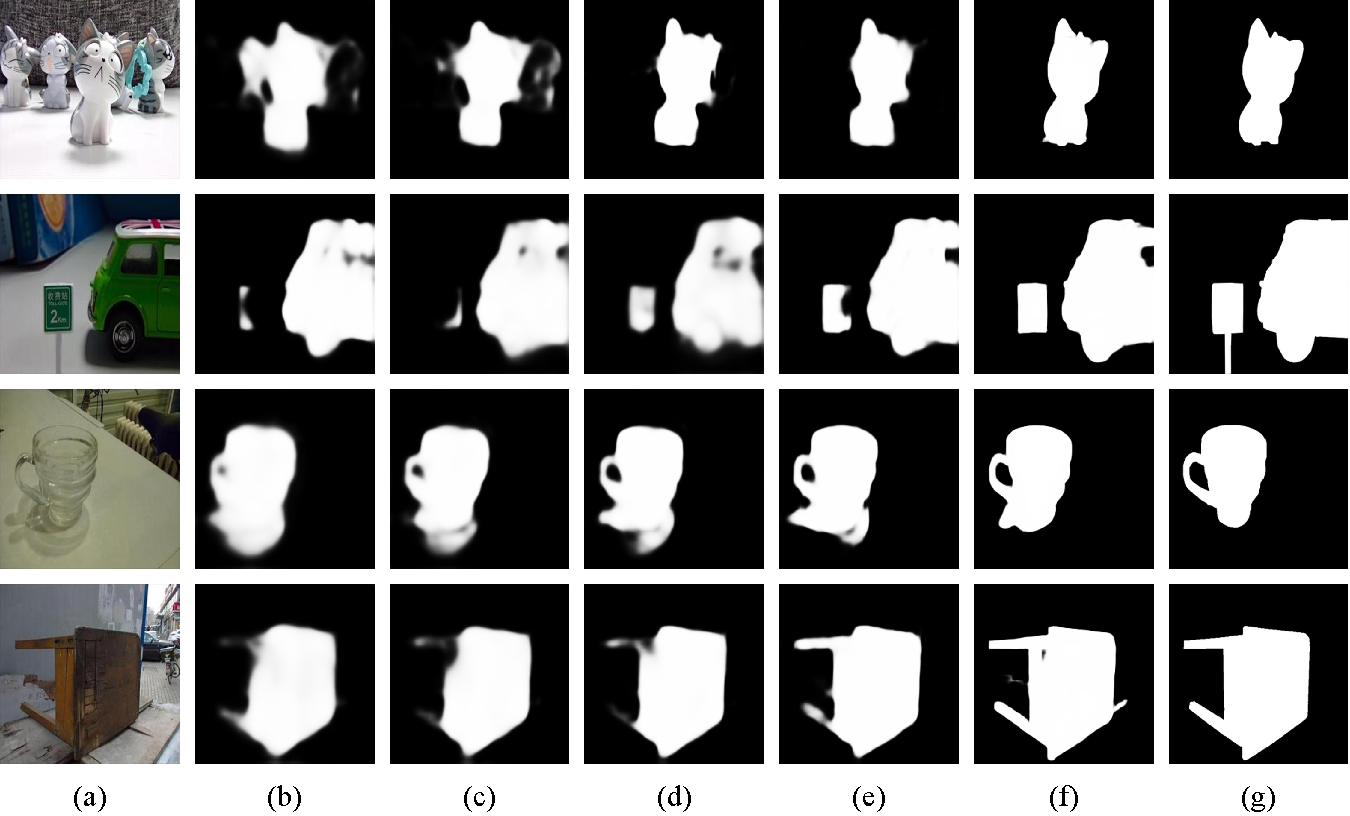
\includegraphics[width=0.99\linewidth]{figures/chapter3/self-comparsion-Use} 
%	\centering
%	
%	
%	%	\caption{   	Visual comparisons of ablation studies.      (a) All-focal images.      
%		%		(b)-(f) Saliency maps of the ``Baseline'', ``+TCM (+TI)'', ``+TCM (++TS)'', ``++FPE'' and ``+++CCM'', respectively.
%		%		%			
%		%		%			(b) Saliency maps of baseline.
%		%		%			(c) Saliency maps w TCM (w/o TS).
%		%		%			(d) Saliency maps w TCM.
%		%		%			(e) Saliency maps w using FPE.
%		%		%			(f) Saliency maps w using CCM.
%		%		(g) Ground truth maps.
%		%	}  
%	%	
%	\bicaption{
%		消融研究的可视化比较。 
%		%	(a) 全聚焦图像,
%		%	(b)-(f) 分别为“基线模型”、
%		%	“+TCM (+TI)”、
%		%	“+TCM (++TS)”、
%		%	“++FPE”和
%		%	“+++CCM图”的显著性图。
%	}{
%		Visual comparisons of ablation studies.      
%		%	(a) All-focal images.      
%		%	(b)-(f) 
%		%	Saliency maps of the ``Baseline'', 
%		%	``+TCM (+TI)'', 
%		%	``+TCM (++TS)'', 
%		%	``++FPE'' and 
%		%	``+++CCM'', respectively.
%		%	(g) Ground truth maps.
%	}
%	\label{figure:self_comp}
%	
%	\vspace{-0.2cm}
%\end{figure}
%
%
















%
%%
%%\par
%\begin{figure}[!ht]
%	\centering
%	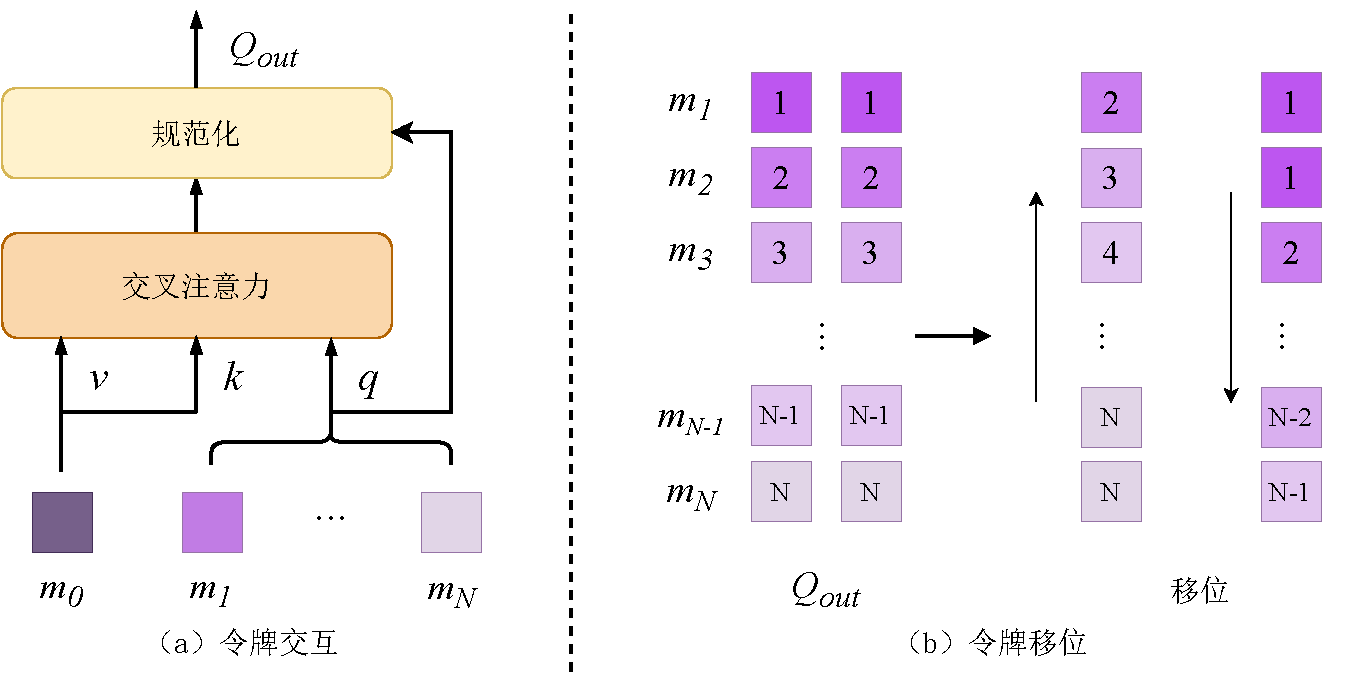
\includegraphics[width=0.95\linewidth]{figures/chapter3/token-interaction.drawio}
%	\bicaption{
%		令牌通信模块 (TCM) 的图示。
%		(a) 令牌交互(TI)。 
%		%		交叉注意力在全焦点和焦点堆栈的嵌入式令牌之间执行特征交互。 
%		(b) 令牌移位(TS)。 
%		%		仅将焦点堆栈流中与焦点相关的标记分成组(图中以2组为例),然后沿焦点深度轴以不同方向(左右)移位以交换切片级信息。
%	}{
%		An illustration of the Token Communication Module (TCM). 
%		(a) Token Interaction (TI). 
%		%	Cross-attention performs feature interactions between the all-focal and focal stack. 
%		(b) Token Shift (TS).
%		%	Only the focus-related tokens in the focus stack stream are split into groups (2 in the figure) and then circularly shifted along the focus-depth axis with different directions to exchange slice-level information.
%	}  
%	\label{cpt3_fig1:token_interaction}
%\end{figure}
%%
%%







%\begin{figure}[!ht]
%	\centering
%	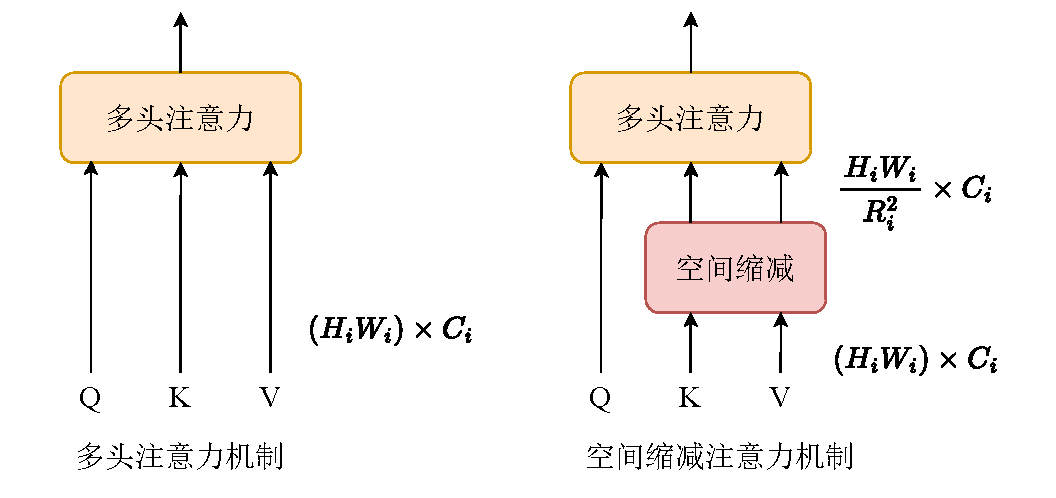
\includegraphics[width=0.95\linewidth]{figures/chapter3/sra}
%	\bicaption{
%		令牌通信模块 (TCM) 的图示。
%		(a) 令牌交互(TI)。 
%		%		交叉注意力在全焦点和焦点堆栈的嵌入式令牌之间执行特征交互。 
%		(b) 令牌移位(TS)。 
%		%		仅将焦点堆栈流中与焦点相关的标记分成组(图中以2组为例),然后沿焦点深度轴以不同方向(左右)移位以交换切片级信息。
%	}{
%		An illustration of the Token Communication Module (TCM). 
%		(a) Token Interaction (TI). 
%		%	Cross-attention performs feature interactions between the all-focal and focal stack. 
%		(b) Token Shift (TS).
%		%	Only the focus-related tokens in the focus stack stream are split into groups (2 in the figure) and then circularly shifted along the focus-depth axis with different directions to exchange slice-level information.
%	}  
%	\label{cpt3_fig1:sra}
%\end{figure}
%%
%%


%
%
%---------------------------------------------------------------------> fig: 创新图
%\begin{figure}[!ht]
%	\centering
%	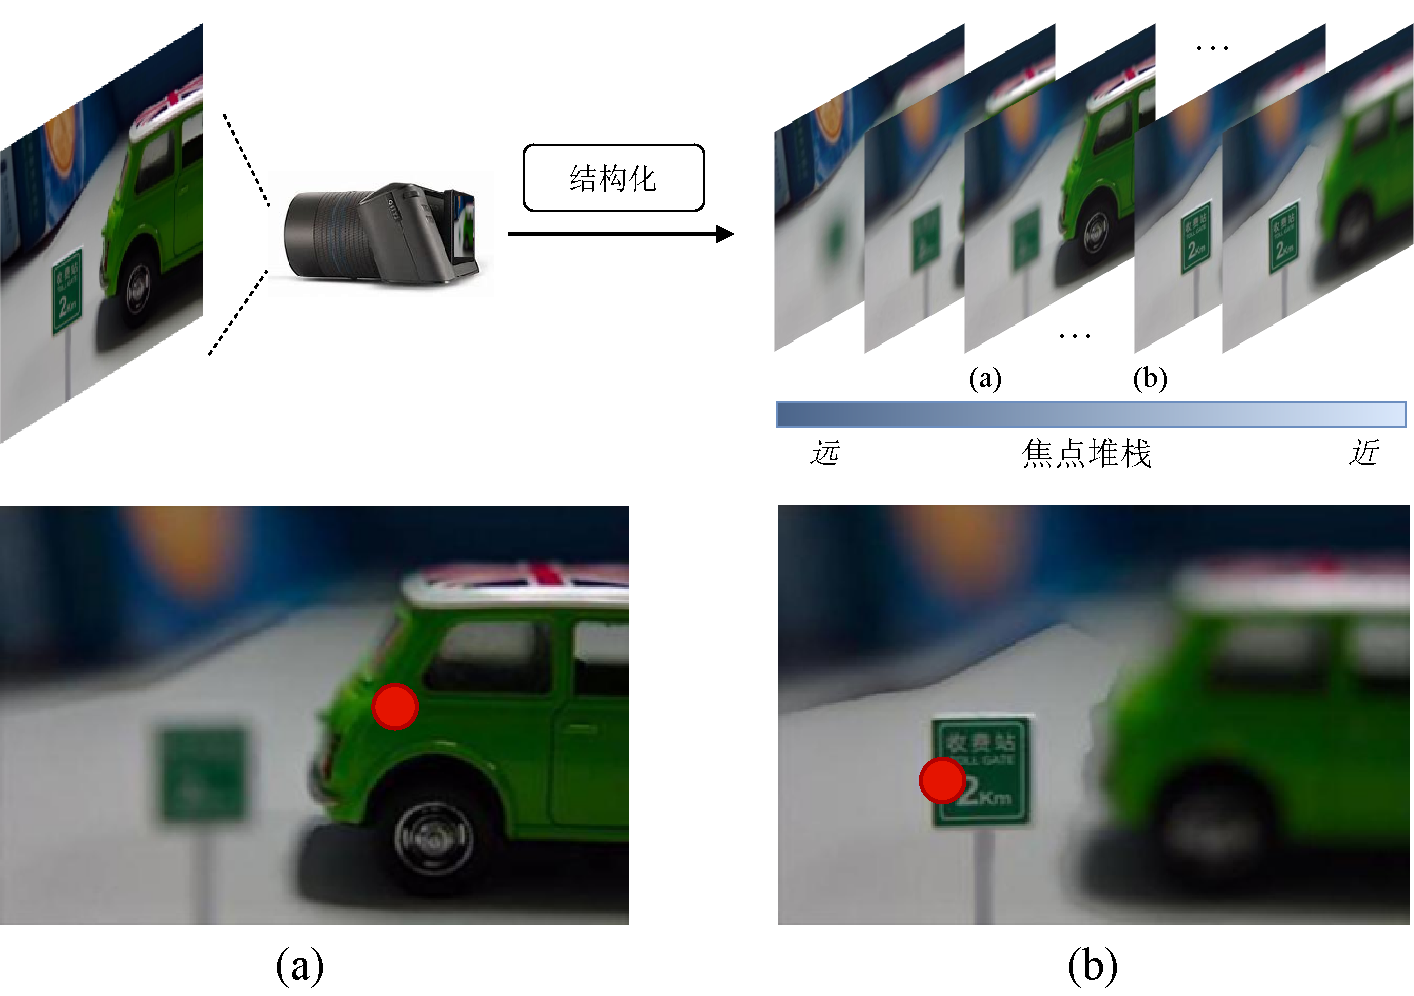
\includegraphics[width=0.85\linewidth]{figures/chapter3/cpt3_idea.pdf}
%	\bicaption{%
%		%		光场焦点堆栈的成像原理和成像效果。
%		%		光场焦点堆栈的成像原理和不同切片的成像效果。
%		光场焦点堆栈的成像过程和不同切片的成像效果。
%		%		\textbf{(a)} 远处视角包含一个清晰的汽车。
%		%		\textbf{(b)} 近处视角包含一个清晰的标志。
%		\textcolor{red}{$\bullet$} 表示清晰的部分。
%		%		焦点堆栈的光场数据结构和焦点堆栈的成像效果的图示。 焦点切片具有随空间透视深度的不同而变化的聚焦部分。
%		%		远处的景色里有一辆清晰的汽车。
%		%		近景画出清晰的标志。
%		%		点表示透明部分。
%	}
%	{ %
%		%			An illustration of the light field data structures to focal stack, and the imaging effect of the focal stack.
%		%			% \textbf{(a)} and \textbf{(b)} indicates that 
%		%			Focal slices have different sharp parts according to the distance from the lens.
%		%			%%
%		%			%%
%		%
%		%% Focal slices have different focusing parts according to the distance from the lens. 
%		%
%		%		An illustration of light field data structures to focal stack and imaging effect of the focal stack. 
%		%		Focal slices have different focusing parts varying with the depth of the spatial perspective.
%		%		The imaging principle and imaging effect of light field focus stack.
%		%		The imaging principle of light field focus stack and the imaging effects of different slices.
%		The imaging process of the light field focus stack and the imaging effects of different slices.
%		%		\textbf{(a)} The distant view contains a clear car.
%		%		\textbf{(b)} The close view draws a clear sign.
%		\textcolor{red}{$\bullet$} indicates the clear parts.  
%	}
%	\label{figure:cpt3:idea}
%\end{figure}
%%
%%


%%------------------------------ figure: comparison
%\begin{figure*}
%	\centering
%	% \setlength{\abovecaptionskip}{-5mm}
%	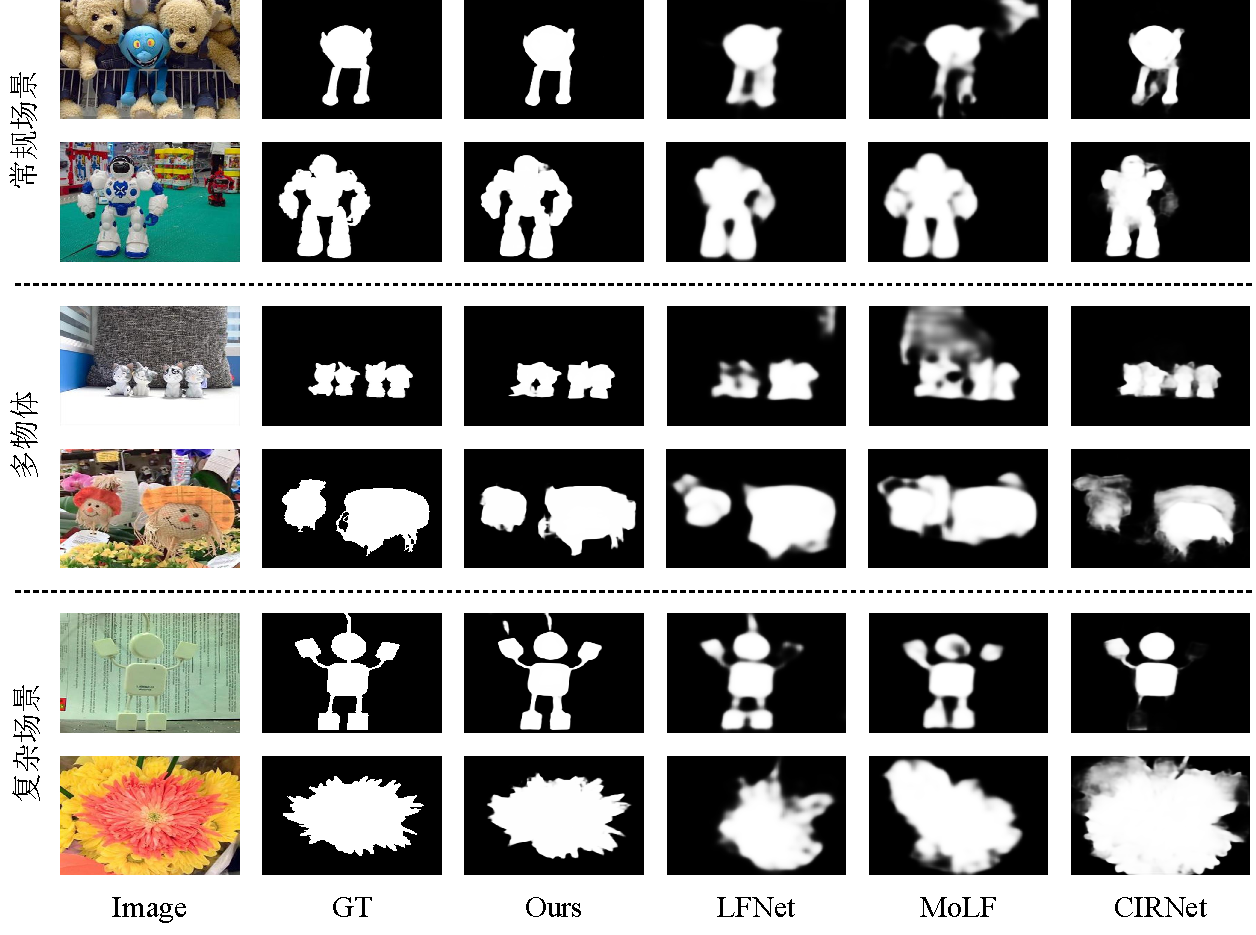
\includegraphics[width=\linewidth]{figures/chapter3/compare_2}
%	%	\caption{
%		%		Qualitative comparisons of state-of-the-art methods in some challenging scenes, including multiple objects and complex scenes.
%		%	}
%	\bicaption{
%		在一些具有挑战性的场景中与最先进的方法的可视化比较。
%	}{
%		Visual comparisons with state-of-the-art methods in challenging scenes.
%		%		Qualitative comparisons of state-of-the-art methods in some challenging scenes, including multiple objects and complex scenes.
%	}
%	\label{figure:figure_comparison_2}
%	\vspace{-0.2cm}
%\end{figure*}
%%
%%

%
%
%	%------------------------------ figure: comparison
%\begin{figure*}
%	\centering
%	% \setlength{\abovecaptionskip}{-5mm}
%	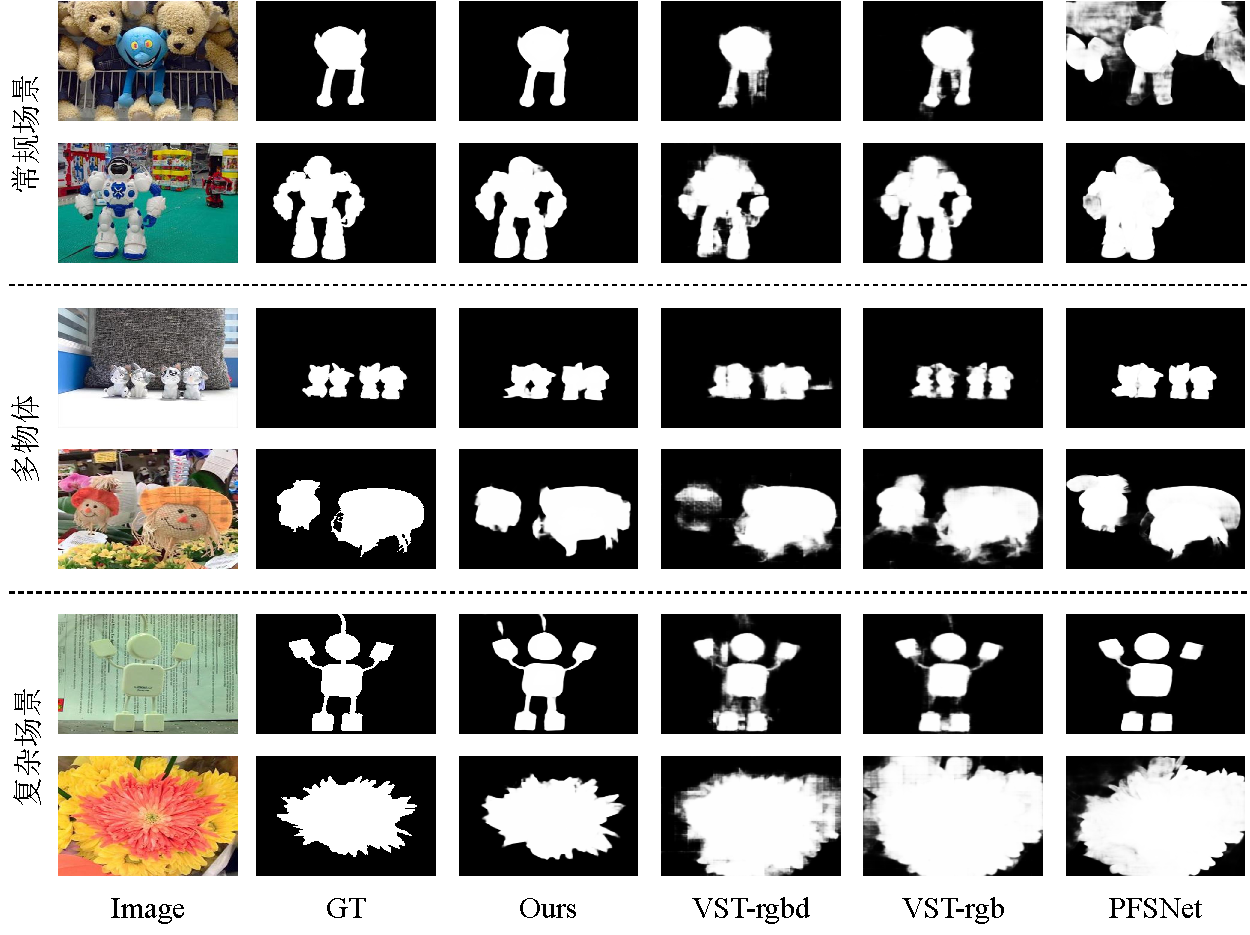
\includegraphics[width=\linewidth]{figures/chapter3/compare_3}
%%	\caption{
	%%		Qualitative comparisons of state-of-the-art methods in some challenging scenes, including multiple objects and complex scenes.
	%%	}
%	\bicaption{
	%		在一些具有挑战性的场景(包括多物体和复杂场景)中对最先进的方法进行定性比较。
	%	}{
	%		Qualitative comparisons of state-of-the-art methods in some challenging scenes, including multiple objects and complex scenes.
	%	}
%	\label{figure:figure_comparison_3}
%	\vspace{-0.2cm}
%\end{figure*}
% 
%



%
%\begin{table}
%	%	\caption{Ablation analyses of each component on the DUTLF-FS dataset.
	%		%		The best results are marked in \textbf{boldface}.
	%		%	}
%	\bicaption{
	%		DUTLF-FS 数据集上每个组件的消融分析。
	%	}{
	%		Ablation analyses of each component on the DUTLF-FS dataset.
	%	}
%	\centering
%	\label{chpt4:tab:abl_2}
%	%	\resizebox{0.82\linewidth}{!}{
	%		\begin{tabular}{llcccc}
		%			\toprule  %添加表格头部粗线
		%			%%  \multicolumn{1}{c}{ \multirow{2}*{Methods} }
		%			
		%			\multicolumn{2}{c}{ \multirow{2}*{Settings}}	& \multicolumn{4}{c}{DUTLF-FS} \\ %& \multicolumn{3}{c}{HFUT} \\ 
		%			
		%			\cmidrule(r){3-6} 
		%			
		%			& & $E_{\phi}^{max}\uparrow$ & $S_{\alpha }\uparrow $ & $F_{\beta}^{max}\uparrow$ & MAE$\downarrow$ \\
		%			\midrule
		%			
		%			% 开始填写数据
		%			\multicolumn{2}{l}{ Baseline }     & 0.947 & 0.894 & 0.901 & 0.048 \\ 
		%			
		%			%		 			\multicolumn{2}{l}{+Token} 	 & 0.959 & 0.918 & 0.926 & 0.037 \\ 
		%			
		%			\midrule
		%			
		%			\multicolumn{1}{c}{ \multirow{2}*{+TCM}}	
		%			
		%			& +TI		& 0.961 & 0.923 & 0.932 & 0.034 \\ 
		%			& ++TS & 0.968 & 0.933 & 0.944 & 0.027 \\
		%			\midrule
		%			
		%			\multicolumn{2}{l}{++FPE} 		& \textbf{0.972} & 0.941 & 0.952 & 0.022 \\
		%			\multicolumn{2}{l}{+++CCM} 		& \textbf{0.972} & \textbf{0.942} & \textbf{0.953} & \textbf{0.021} \\ 
		%			
		%			
		%			\bottomrule
		%		\end{tabular}
	%		% }
%\end{table}
%
%\begin{table}
%	%	\caption{Ablation analyses of each component on the DUTLF-FS dataset.
	%		%		The best results are marked in \textbf{boldface}.
	%		%	}
%	\bicaption{
	%		DUTLF-FS 数据集上每个组件的消融分析。
	%	}{
	%		Ablation analyses of each component on the DUTLF-FS dataset.
	%	}
%	\centering
%	\label{chpt4:tab:abl_3}
%	%	\resizebox{0.82\linewidth}{!}{
	%		\begin{tabular}{llcccc}
		%			\toprule  %添加表格头部粗线
		%			%%  \multicolumn{1}{c}{ \multirow{2}*{Methods} }
		%			
		%			\multicolumn{2}{c}{ \multirow{2}*{Settings}}	& \multicolumn{4}{c}{DUTLF-FS} \\ %& \multicolumn{3}{c}{HFUT} \\ 
		%			
		%			\cmidrule(r){3-6} 
		%			
		%			& & $E_{\phi}^{max}\uparrow$ & $S_{\alpha }\uparrow $ & $F_{\beta}^{max}\uparrow$ & MAE$\downarrow$ \\
		%			\midrule
		%			
		%			% 开始填写数据
		%			\multicolumn{2}{l}{ Baseline }     & 0.947 & 0.894 & 0.901 & 0.048 \\ 
		%			
		%			%		 			\multicolumn{2}{l}{+Token} 	 & 0.959 & 0.918 & 0.926 & 0.037 \\ 
		%			
		%			\midrule
		%			
		%			\multicolumn{1}{c}{ \multirow{2}*{+TCM}}	
		%			
		%			& +TI		& 0.961 & 0.923 & 0.932 & 0.034 \\ 
		%			& ++TS & 0.968 & 0.933 & 0.944 & 0.027 \\
		%			\midrule
		%			
		%			\multicolumn{2}{l}{++FPE} 		& \textbf{0.972} & 0.941 & 0.952 & 0.022 \\
		%			\multicolumn{2}{l}{+++CCM} 		& \textbf{0.972} & \textbf{0.942} & \textbf{0.953} & \textbf{0.021} \\ 
		%			
		%			
		%			\bottomrule
		%		\end{tabular}
	%		% }
%\end{table}




然而,







\todo






大小为原始分别率的

我们的视角增强注意力模块,














% 
% 
在这里,$M_{l-1} \in \left \{  0,1\right \} ^{N \times H_{l}W_{l}} $是前一个
$l-1$层和
\textcolor{red}{TODO}
$M_{0}$是在将查询特征输入Transformer解码器之前,从全聚焦支路获得的二进制掩码预测。
%
%
%
%
\par 
%
%
%











\BiSection{uuu}{uuu}

像素级交叉熵损失。



之后分割头$f_{SEG}$把图像$I$映射到分类激活图
$Y=f_{SEG}(I) \in \mathbb{R}^{H\times H \times |C|}$。
进一步设$y=\left [ y_{1},\dots, y_{C} \right ] \in\mathbb{R}^{C}$
是像素$i$的非归一化得分向量(称为logit),可以从$Y$导出,
即$y \in Y$。
给定像素$i$的真实标签$\bar{c} \in C$,交叉熵使用softmax进行优化:
\begin{equation}
	\mathcal{L}_{i}^{CE}=-1_{\bar{c}}^{\top } log(softmax(y))
	\label{chpt4:eq:loss_softmax}
\end{equation}
% 
% 
% 
% 
其中,$1_{\bar{c}}$表示$\bar{c}$的one-hot编码,
其中的对数算法是逐元素计算的:
\begin{equation}
	softmax(y_{c}) = \frac
	{exp(y_{c})}
	{ 
		\sum_{{c}'=1 }^{|C|} 
		exp(y_{{c}'}) 
	} 
\end{equation}
% 
% 
% 
% 
这种独立训练目标的设计有两个主要限制。
1)它独立的乘法像素级预测,但忽略像素之间的关系~\cite{zhao2019region}。
2)由于使用了softmax,损失仅取决于logits之间的相对关系,
不能直接得到监督学习的表示~\cite{pang2019rethinking}。
这两个问题很少被注意到;只有少数结构感知损失被设计来解决1),
通过考虑像素亲和力~\cite{ke2018adaptive},
优化交叉测量~\cite{berman2018lovasz},
或者最大化真值和预测图之间的互信息~\cite{zhao2019region}。然而,
这些替代损失仅考虑图像内像素之间的依赖性(即全局上下文),
而不考虑图像不同像素之间的语义相关性(即全局结构)
\par
% 
% 
% 
% 

\par
% 
% 


稍后在\todo 和\todo 中提供了定量分析。


像素与区域的对比。
如\todo 所述,记忆是一项关键技术,
有助于对比学习利用海量数据来学习良好的表示。
然而,由于我们的密集预测设置中有大量的像素样本,
并且其中大多数是冗余的(即从相似对象区域采样),
因此像传统存储器一样直接存储所有训练像素样本\todo ,
会大大减慢学习过程。
\par
% 
% 
% 
% 
在队列中维护最后几个批次,例如\todo,
也不是一个最优的选择,
因为最近的批次仅包含有限数量的图像,
降低了像素样本的多样性。
因此,我们选择分别为前景类和背景类维护一个像素队列。
对于每个类别,仅从最新小批量中的每个图像中随机选择少量像素$V$,
并将其拉如队列,大小为$T \gg  V$。
% 
% 
% 
% 
在实践中,我们发现这种策略非常高效并且有效,但是欠采样像素嵌入
太稀疏,无法完全捕获图像内容。
因此,我们进一步构建了一个区域存储库,用于存储从图像片段(即语义区域)
吸收的更具代表性的嵌入。


具体来说,对于总共有$N$个训练图像和$|C|=2$个分割类,
我们的区域内存的大小为$|C|\times N \times D$,
其中$D$是像素嵌入的维度。区域内存中的第$(\bar{c},~n)$
个元素是通过平均池化第n个图像中标记为$c$类别的像素的所有嵌入而获得的
$D$维特征向量。
使用区域内存有两个优点:

1)以较低的内存消耗存储更具代表性的像素样本;
2)允许我们的像素对比损失~\ref{chpt4:eq:con_loss}~进一步探索像素与区域的关系。
关于2),当计算属于$\bar{c}$类别的锚像素$i$时,计算公式~\ref{chpt4:eq:con_loss}~时,
具有相同类别$\bar{c}$的存储区域嵌入被视为正例,
而具有其他类别$C/ \bar{c}$ 的区域嵌入被视为负例。
% 
% 
% 
% 
\par
对于像素存储器,大小为$|C|\times T \times D$。
因此,对于整个内存(记为 $M$ )来说,总大小为$|C| \times (N+T) \times D$。
在\todo 中检查了$M$ 中的像素嵌入和区域嵌入。




\todo 
















%
% 

%
%
%
\par
% 
% 
% 
% 

\par

\par
% 
% 
% 
% 

因此,引入了一种有效的多尺度策略,在控制计算量增加的同时,引入高分辨率特征。
首先,由最高层分辨率特征和下两层较低的分辨率特征组成特征金字塔,
并一次将多尺度的特征的一个分辨率特征传递给一个Transformer解码器层。
\par
% 
% 





Transformer有两个已知的问题。
一是Transformer需要很长的训练时间才能收敛。
假设查询和关键元素的数量分别为$N_{q}$和$N_{k}$,
通过适当的参数初始化,$U_{m}z_{q}$和$ V_{m}x_{k}$遵循均值为0,方差为1的分布,
这使得当$N_{k}$很大时,
注意力权重$A_{mqk} \approx \frac{1}{N_{k}} $。
它将导致输入特征的梯度不明确。
因此,需要很长的训练计划,以便注意力权重可以集中在特定的键上。
在图像领域中,关键元素通常是图像像素,$N_{k}$可能非常大,并且很难收敛。
% 
% 
% 
% 
\par
%
% 
% 
% 
另一方面,由于存在大量查询和关键元素,多头注意力的计算和内存复杂度可能非常高。
方程的计算复杂度为$O\left ( N_{q}C^{2} + N_{k}C^{2}+N_{q}N_{k}C \right ) $。
在图像领域中,查询元素和关键元素都是像素,$N_{q}=N_{k} \gg C$,
复杂度由第三项主导,即$O(N_{q}N_{k}C) $。
因此,多头注意力模块的复杂度随着特征图大小呈二次方增长。


可变形注意力模块。

在图像特征图上应用Transformer的核心问题是让它会查看所有可能得空间位置。
为了解决这个问题,我们采用了一个可变形的注意力模块。
受可变形卷积的启发,
可变形注意力模块仅关注参考点周围的一小组关键采样点,
而不管特征图的空间大小,
通过为每个查询仅分配少量固定数量的键,可以环节收敛和特征空间分辨率的问题。


给定输入特征图$x \in \mathbb{R}^{C\times H \times W}$,
令$q$用作为内容特征$z_{q}$和二维参考点$p_{q}$的索引查询元素,可变性卷积特征
通过以下方式计算,
% 
% 
% 
% 
\begin{equation}
	DeformAttn(z_{q},~p_{q},x)=
	\sum_{m=1}^{M}
	W_{m}\left [ 
	\sum_{k=1}^{K}A_{mqk}~\cdot~
	W_{m}^{'}x\left ( p_{q} + \bigtriangleup p_{mqk} \right ) 
	~~\right ]  
\end{equation}
% 
% 
% 
% 
其中$m$索引注意力头,$k$索引采样键,
$K$是采样键的总数($K \ll HW$),
$\bigtriangleup p_{mqk} $和$A_{mqk}$分别表示
第$m^{th}$个注意力头中第$k^{th}$个采样点的采样偏移量和注意力权重。
标量注意力权重$A_{mqk}$位于$\left [ 0,~1 \right ] $范围内,
通过$ {\textstyle \sum_{k=1}^{K}} A_{mqk}=1$进行归一化。
$\bigtriangleup p_{mqk} \in \mathbb{R}^{2}$
是范围不受约束的二维实数。
由于$p_{q} + \bigtriangleup p_{mqk}$是分数,如等人所述,
$x\left ( p_{q} + \bigtriangleup p_{mqk} \right ) $在计算时应用双线性插值。
$\bigtriangleup p_{mqk}   $和$A_{mqk}$都是通过查询特征$z_{q}$上的线性投影获得的。
在具体实现中,查询特征$z_{q}$被馈送到$3MK$通道的线性投影算子,
其中前$2MK$通道对采样偏移量$\bigtriangleup p_{mqk}$进行编码,
其余$MK$通道通过被馈送到$softmax$算子以获得注意力权重$A_{mqk}$。





可变形注意力模块旨在将卷积特征图作为关键元素进行处理。

设 为查询元素的数量,当较小时,可变形注意力模块的复杂度为。
当应用于DETR编码器时,其中,复杂度变为,
起复杂度与空间大小呈线性关系。
当它作为DETR解码器中的交叉注意力模块应用时,
其中,是对象查询的数量,复杂度变为,
这与空间大小无关。


多尺度可变形注意力模型。
大多数现代目标检测框架都受益于多尺度特征图。
我们提出的可变形注意力模块可以自然地扩展到多尺度特征图。
令为输入多尺度特征图,
其中。
令为每个查询元素的参考点的归一化坐标,
然后应用多尺度可变形注意力采样点。
分别表示第几个特征层和第几个注意力头中第几个采样点的采样偏移和注意力权重。
标量注意力权重通过进行归一化。

这里,为了尺度公式的清晰性,我们使用归一化坐标,
其中归一化坐标分别表示图像的左上角和右下角。
方程中的函数将归一化坐标重新放缩到第几层的输入特征图。


多尺度可变形注意力与之前的单尺度版本非常相似,只是它从多尺度特征图中采样点,
而不是从单尺度特征图中采样k个点。
当且固定为单位矩阵时,所提出的注意力模块将退化为可变形卷积。
可变形卷积是针对单尺度输入而设计的,每个注意力头仅关注一个采样点。
然而,我们的多尺度可变形注意力会关注来自多尺度输入的多个采样点。
所提出的(多尺度)可变形注意模块也可以被视为
Transformer 注意的有效变体,其中通过可变形采样位置引入预过滤机制。
当采样点遍历所有可能得位置时,所提出的注意力模块相当于Transformer注意力。


可变形Transformer 编码器。

我们将网络中处理特征图的Transformer注意模块替换为所提出的多尺度可变形注意模块。
编码器的输入和输出都是具有相同分辨率的多尺度特征图。

在编码器中,我们从骨干网络中提取多尺度特征图,通过卷积,
其中的分辨率比输入图像低。
最低分辨率特征图是通过最后阶段的步长卷积获得的。

所有多尺度特征图均为个通道,
像FPN网络结构中,没有使用自上而下的结构,因为我们提出的多尺度可变形注意力本身可以在多尺度特征图之间交换信息。






%
%\begin{table*}[]
%	%
%	%---------------------------------------------------------------------> 大表 
%	%
%	\caption{Quantitative comparison of our proposed FPT with other 20 SOTA SOD methods on three benchmark datasets. 
	%		$ \uparrow \& \downarrow $ denote larger and smaller is better.
	%		%
	%		% denote the best and the second-best results,
	%		%
	%		The best three results are shown in 
	%		\textbf{boldface}, \textcolor{red}{red} and \textcolor{blue}{blue} fonts respectively. 
	%		% '-' indicates the code or outcome is not available.
	%	}
%	\centering
%	\label{table:comp_with_sota_1}
%%	\resizebox{\textwidth}{!}{
	%		\begin{tabular}{crcccc}
		%			\toprule  %添加表格头部粗线
		%			
		%			% title
		%			\multirow{2}*{Type} & \multicolumn{1}{c}{ \multirow{2}*{Methods} } & 
		%			\multicolumn{4}{c}{DUTLF-FS \cite{zhang2019memory} } \\
		%
		%			
		%			% next line
		%			\cmidrule(r){3-6} 
		%			
		%			% subtitle
		%			& & 
		%			$E_{\phi}^{max}\uparrow$ & $S_{\alpha }\uparrow$ & $F_{\beta}^{max}\uparrow$ & MAE$\downarrow$ \\
		%		
		%			
		%			% line line
		%			\midrule
		%			
		%			\multirow{8}*{\textit{Light field}}
		%			
		%			% 开始填数据
		%			
		%			& Ours	 &  {\textbf{0.973}} & \textbf{ {0.946}} 
		%			& \textbf{ {0.954}} & \textbf{ {0.020}} 
		%			\\
		%			
		%			& DLGLRG \cite{liu2021light} 
		%			& {\textcolor{red}{0.958}} & {\textcolor{red}{0.928}} 
		%			& {\textcolor{red}{0.934}} & {\textcolor{red}{0.029}} 
		%			\\
		%			
		%			& ERNet \cite{piao2020exploit}
		%			& 0.947 & 0.899 & 0.908 & 0.039  \\
		%			
		%			& PANet \cite{piao2021panet} 
		%			% & 0.9390 & 0.9080 & 0.9029 & 0.0383 & 0.8449 & 0.7949 & 0.7383 & 0.0743 & 0.8922 & 0.8487 & 0.8494 & 0.0761 
		%			& 0.939 & 0.908 & 0.903 & 0.038
		%			\\
		%			
		%			& LFNet	 \cite{zhang2020lfnet} 
		%			& 0.929 & 0.878 & 0.890 & 0.053 	 \\
		%			
		%			& MAC	 \cite{zhang2020light} 
		%			& 0.863	& 0.804	& 0.792	& 0.102	    \\
		%			
		%			& MoLF	 \cite{zhang2019memory} 
		%			& 0.938 & 0.887 & 0.902 & 0.051 	 \\
		%			
		%			& DLSD	\cite{piao2019deep}
		%			& 0.891	& 0.841	& 0.801	& 0.076	    \\
		%			
		%			\midrule % end lfsod
		%			
		%			% start rgb-d
		%			\multirow{6}*{\textit{RGB-D}}
		%			
		%			% & 001& Male & 001& Male& 001& Male& 001& Male& 001& Male & 001& Male  & 001& Male \\
		%			
		%			& DCF \cite{ji2021calibrated} 
		%			& \textcolor{blue}{0.954} & \textcolor{blue}{0.921} & \textcolor{blue}{0.927} & \textcolor{blue}{0.031} 
		%		 	\\
		%			
		%			& CIR-Net \cite{cong2022cir}
		%			& 0.950 & 0.916 & 0.921 & 0.038 
		%		    \\ 
		%			
		%			& VST-$rgbd$  \cite{liu2021visual} 
		%			& 0.952 & 0.920 & 0.921 & 0.036 
		%			\\
		%			
		%			
		%			& BBS-Net     \cite{fan2020bbs} 
		%			& 0.900 & 0.865 & 0.852 & 0.066 
		%			\\ 
		%			
		%			& SSF     \cite{zhang2020select} 
		%			& 0.922 & 0.879 & 0.887 & 0.050 
		%			\\ 
		%			
		%			& S2MA    \cite{liu2020learning} 
		%			& 0.839 & 0.787 & 0.754 & 	0.102 
		%			\\
		%			
		%			\midrule % end rgb-d
		%			
		%			\multirow{7}*{\textit{RGB}}
		%			
		%			& VST-$rgb$ \cite{liu2021visual} 
		%			& 0.939 & 0.910 & 0.911 & 0.047  \\ 
		%			
		%			& PFSNet \cite{ma2021pyramidal}
		%			& 0.912 & 0.883 & 0.879 & 0.057  \\ 
		%			
		%			& ITSD \cite{zhou2020interactive} & 
		%			0.930 & 0.899 & 0.899 & 0.052  \\ 
		%			
		%			
		%			
		%			& LDF \cite{wei2020label} &
		%			0.898 & 0.873 & 0.861 & 0.061 \\ 
		%			
		%			
		%			& MINet \cite{pang2020multi} &
		%			0.916 & 0.890 & 0.882 & 0.050  \\ 
		%			
		%			& F$^{3}$Net  \cite{wei2020f3net}
		%			& 0.900 & 0.888 & 0.882 & 0.057  \\ 
		%			
		%			& EGNet   \cite{zhao2019egnet}
		%			& 0.914 & 0.886 & 0.870 & 0.053 \\ 
		%			
		%			\bottomrule % end
		%	\end{tabular}
	%%}
%\end{table*}
%
%
%
%\begin{table*}[]
%	%
%	%---------------------------------------------------------------------> 大表 
%	%
%	\caption{Quantitative comparison of our proposed FPT with other 20 SOTA SOD methods on three benchmark datasets. 
	%		$ \uparrow \& \downarrow $ denote larger and smaller is better.
	%		%
	%		% denote the best and the second-best results,
	%		%
	%		The best three results are shown in 
	%		\textbf{boldface}, \textcolor{red}{red} and \textcolor{blue}{blue} fonts respectively. 
	%		% '-' indicates the code or outcome is not available.
	%	}
%	\centering
%	\label{table:comp_with_sota_2}
%%	\label{table:comp-with-sota}
%%	\resizebox{\textwidth}{!}{
	%		\begin{tabular}{crcccc}
		%			\toprule  %添加表格头部粗线
		%			
		%			% title
		%			\multirow{2}*{Type} & \multicolumn{1}{c}{ \multirow{2}*{Methods} } & 
		%			\multicolumn{4}{c}{HFUT \cite{zhang2017saliency} } \\
		%			
		%			% next line
		%			\cmidrule(r){3-6} 
		%			
		%			% subtitle
		%			& & 
		%			$E_{\phi}^{max}\uparrow$ & $S_{\alpha }\uparrow$ & $F_{\beta}^{max}\uparrow$ & MAE$\downarrow$ \\
		%			
		%			% line line
		%			\midrule
		%			
		%			\multirow{8}*{\textit{Light field}}
		%			
		%			% 开始填数据
		%			
		%			& Ours	 
		%			& \textbf{ {0.871}} &	\textbf{ {0.828}} 
		%			&\textbf{	 {0.784}} & {\textcolor{red}{0.064}} 
		%		    \\
		%			
		%			& DLGLRG \cite{liu2021light} 
		%			&	0.839 &	0.766 &	0.698 &	0.070 
		%	        \\
		%			
		%			& ERNet \cite{piao2020exploit}
		%			&	0.841 &	0.778 &	0.722 &	0.082 \\
		%			
		%			& PANet \cite{piao2021panet} 
		%			% & 0.9390 & 0.9080 & 0.9029 & 0.0383 & 0.8449 & 0.7949 & 0.7383 & 0.0743 & 0.8922 & 0.8487 & 0.8494 & 0.0761 
		%			& 0.845 & 0.795 & 0.738 & 0.074 
		%			\\
		%			
		%			& LFNet	 \cite{zhang2020lfnet} 
		%			&	0.846 &	0.782 &	0.718 &	0.073 \\
		%			
		%			& MAC	 \cite{zhang2020light} 
		%			&   0.797 & 0.731 & 0.667 & 0.107 
		%			\\
		%			
		%			& MoLF	 \cite{zhang2019memory} 
		%			&	0.852 &	0.789 &	0.729 &	0.075 \\
		%			
		%			& DLSD	\cite{piao2019deep}
		%			&   0.783 & 0.741 & 0.615 & 0.098 \\
		%			
		%			
		%			\midrule % end lfsod
		%			
		%			\multirow{6}*{\textit{RGB-D}}
		%
		%			
		%			& DCF \cite{ji2021calibrated} 
		%			& \textcolor{blue}{0.856} & {\textcolor{red}{0.812}} & {\textcolor{red}{0.768}} & \textcolor{blue}{0.065} 
		%			\\
		%			
		%			& CIR-Net \cite{cong2022cir}
		%			& {\textcolor{red}{0.862}} & 0.800 
		%			& 0.742 & \textbf{ {0.062}} 
		%			\\ 
		%			
		%			& VST-$rgbd$  \cite{liu2021visual} 
		%			& 0.843 & 0.807 & 0.754 & 0.086  \\
		%
		%			
		%			& BBS-Net     \cite{fan2020bbs} 
		%			& 0.801 & 0.751 & 0.676 & 0.073 
		%			\\ 
		%			
		%			& SSF     \cite{zhang2020select} 
		%			& 0.816 & 0.725 & 0.647 & 0.090 
		%		    \\ 
		%			
		%			& S2MA    \cite{liu2020learning} 
		%		    & 0.777 & 0.729 & 0.650 & 0.112 \\
		%			
		%			
		%			%			& TriTransNet	&  & \\
		%			%			& DCFNet  & \\
		%			
		%			\midrule % end rgb-d
		%			
		%			% start rgb sod
		%			\multirow{7}*{\textit{RGB}}
		%			
		%			& VST-$rgb$ \cite{liu2021visual} 
		%			& 0.831 & \textcolor{blue}{0.808} & \textcolor{blue}{0.763} & 0.093 \\ 
		%			
		%			& PFSNet \cite{ma2021pyramidal}
		%			&  0.835 & 0.800 & 0.752 & 0.088  \\ 
		%			
		%			%			& - & \\
		%			
		%			& ITSD \cite{zhou2020interactive} & 
		%			 0.839 & 0.805 & 0.759 & 0.089  \\ 
		%			
		%			
		%			
		%			& LDF \cite{wei2020label} &
		%			 0.804 & 0.780 & 0.708 & 0.093  \\ 
		%			
		%			
		%			& MINet \cite{pang2020multi} 
		%			 & 0.816 & 0.792 & 0.720 & 0.086  \\ 
		%			
		%			& F$^{3}$Net  \cite{wei2020f3net}
		%			& 0.815 & 0.777 & 0.718 & 0.095  \\ 
		%
		%			
		%			& EGNet   \cite{zhao2019egnet}
		%			 & 0.794 & 0.772 & 0.672 & 0.094  \\ 
		%			
		%			\bottomrule % end
		%	\end{tabular}
	%%}
%\end{table*}


%
%\begin{table*}[]
%	%
%	%---------------------------------------------------------------------> 大表 
%	%
%	\caption{Quantitative comparison of our proposed FPT with other 20 SOTA SOD methods on three benchmark datasets. 
	%		$ \uparrow \& \downarrow $ denote larger and smaller is better.
	%		%
	%		% denote the best and the second-best results,
	%		%
	%		The best three results are shown in 
	%		\textbf{boldface}, \textcolor{red}{red} and \textcolor{blue}{blue} fonts respectively. 
	%		% '-' indicates the code or outcome is not available.
	%	}
%	\centering
%	\label{table:comp_with_sota_3}
%%	\label{table:comp-with-sota}
%%	\resizebox{\textwidth}{!}{
	%		\begin{tabular}{crcccc}
		%			\toprule  %添加表格头部粗线
		%			
		%%			\multirow{2}*{Type} & 
		%			\multicolumn{1}{c}{ \multirow{2}*{Methods} } & 
		%			% \multirow{2}*{Years} &
		%			% \multicolumn{1}{c}{Type} & \multicolumn{1}{c}{Methods} & \multicolumn{1}{c}{Years} & 
		%			\multicolumn{4}{c}{DUTLF-FS \cite{zhang2019memory} } &
		%			\multicolumn{4}{c}{HFUT \cite{zhang2017saliency} } &
		%			\multicolumn{4}{c}{LFSD \cite{li2014saliency} } \\
		%			
		%			% next line
		%			\cmidrule(r){2-5} \cmidrule(r){6-9} \cmidrule(r){10-13}
		%			
		%			% subtitle
		%			& 
		%			$E_{\phi}^{max}\uparrow$ & $S_{\alpha }\uparrow$ & $F_{\beta}^{max}\uparrow$ & MAE$\downarrow$ &
		%			$E_{\phi}^{max}\uparrow$ & $S_{\alpha }\uparrow$ & $F_{\beta}^{max}\uparrow$ & MAE$\downarrow$  &
		%			$E_{\phi}^{max}\uparrow$ & $S_{\alpha }\uparrow$ & $F_{\beta}^{max}\uparrow$ & MAE$\downarrow$ \\
		%			
		%			
		%			% line line
		%			\midrule
		%			
		%			\multirow{8}*{\textit{Light field}}
		%			
		%			% 开始填数据
		%			
		%			& Ours	 
		%%			&  {\textbf{0.973}} & \textbf{ {0.946}} 	& \textbf{ {0.954}} & \textbf{ {0.020}} 
		%%			& \textbf{ {0.871}} &	\textbf{ {0.828}} 			&\textbf{	 {0.784}} & {\textcolor{red}{0.064}} 
		%			& \textbf{ {0.919}} &	\textcolor{blue}{0.860} 			&	\textbf{ {0.873}} &	\textbf{ {0.064}} 
		%			\\
		%			
		%			& DLGLRG \cite{liu2021light} 
		%%			& {\textcolor{red}{0.958}} & {\textcolor{red}{0.928}} 			& {\textcolor{red}{0.934}} & {\textcolor{red}{0.029}} 
		%%			&	0.839 &	0.766 &	0.698 &	0.070 
		%			&	{\textcolor{red}{0.906}} &	\textbf{ {0.866}} 			&	{\textcolor{red}{0.870}} &	\textcolor{blue}{0.069} 
		%			\\
		%			
		%			& ERNet \cite{piao2020exploit}
		%%			& 0.947 & 0.899 & 0.908 & 0.039 
		%%			&	0.841 &	0.778 &	0.722 &	0.082 
		%			&	0.888 &	0.834 &	0.850 &	0.082 
		%			\\
		%			
		%			& PANet \cite{piao2021panet} 
		%%			& 0.939 & 0.908 & 0.903 & 0.038 
		%%			& 0.845 & 0.795 & 0.738 & 0.074 
		%			& 0.892 & 0.849 & 0.849 & 0.076
		%			\\
		%			
		%			& LFNet	 \cite{zhang2020lfnet} 
		%%			& 0.929 & 0.878 & 0.890 & 0.053
		%%			 &	0.846 &	0.782 &	0.718 &	0.073 
		%			 &	0.885 &	0.820 &	0.824 &	0.092 \\
		%			
		%			& MAC	 \cite{zhang2020light} 
		%%			& 0.863	& 0.804	& 0.792	& 0.102	
		%%			&   0.797 & 0.731 & 0.667 & 0.107 
		%			& 0.832 & 0.782 & 0.776 & 0.127 \\
		%			
		%			& MoLF	 \cite{zhang2019memory} 
		%%			& 0.938 & 0.887 & 0.902 & 0.051 
		%%			&	0.852 &	0.789 &	0.729 &	0.075 
		%			&	0.888 &	0.830 &	0.834 &	0.089 \\
		%			
		%			& DLSD	\cite{piao2019deep}
		%%			& 0.891	& 0.841	& 0.801	& 0.076	
		%%			&   0.783 & 0.741 & 0.615 & 0.098 
		%			& 0.806 & 0.737 & 0.715 & 0.147 \\
		%			
		%			\midrule % end lfsod
		%			
		%			% start rgb-d
		%			\multirow{6}*{\textit{RGB-D}}
		%			
		%			& DCF \cite{ji2021calibrated} 
		%%			& \textcolor{blue}{0.954} & \textcolor{blue}{0.921} & \textcolor{blue}{0.927} & \textcolor{blue}{0.031} 
		%%			& \textcolor{blue}{0.856} & {\textcolor{red}{0.812}} & {\textcolor{red}{0.768}} & \textcolor{blue}{0.065} 
		%			& 0.881 & 0.809 & 0.821 & 0.096 \\
		%			
		%			& CIR-Net \cite{cong2022cir}
		%%			& 0.950 & 0.916 & 0.921 & 0.038 
		%%			& {\textcolor{red}{0.862}} & 0.800  			& 0.742 & \textbf{ {0.062}} 
		%			& 0.874 & 0.820 & 0.816 & 0.098 \\ 
		%			
		%			& VST-$rgbd$  \cite{liu2021visual} 
		%%			& 0.952 & 0.920 & 0.921 & 0.036 
		%%			& 0.843 & 0.807 & 0.754 & 0.086 
		%			& 0.851 & 0.792 & 0.786 & 0.110 
		%			\\
		%			
		%			%			& -  & 2022  & \\
		%			%			& -  & 2022  & \\
		%			
		%			& BBS-Net     \cite{fan2020bbs} 
		%%			& 0.900 & 0.865 & 0.852 & 0.066 
		%%			& 0.801 & 0.751 & 0.676 & 0.073 
		%			& \textcolor{blue}{0.901} & {\textcolor{red}{0.864}} & 0.858 & 0.072 \\ 
		%			
		%			& SSF     \cite{zhang2020select} 
		%%			& 0.922 & 0.879 & 0.887 & 0.050 
		%%			& 0.816 & 0.725 & 0.647 & 0.090 
		%			& \textcolor{blue}{0.901} & 0.859 & \textcolor{blue}{0.868} & {\textcolor{red}{0.067}} \\ 
		%			
		%			& S2MA    \cite{liu2020learning} 
		%%			& 0.839 & 0.787 & 0.754 & 	0.102 
		%%			& 0.777 & 0.729 & 0.650 & 0.112 
		%			& 0.873 & 0.837 &	0.835 & 0.094 \\
		%
		%			
		%			\midrule % end rgb-d
		%			\multirow{7}*{\textit{RGB}}
		%			
		%			& VST-$rgb$ \cite{liu2021visual} 
		%%			& 0.939 & 0.910 & 0.911 & 0.047
		%%			& 0.831 & \textcolor{blue}{0.808} & \textcolor{blue}{0.763} & 0.093 
		%			& 0.865 & 0.797 & 0.817 & 0.123 
		%			\\ 
		%			
		%			& PFSNet \cite{ma2021pyramidal}
		%%			& 0.912 & 0.883 & 0.879 & 0.057 
		%%			& 0.835 & 0.800 & 0.752 & 0.088 
		%			& 0.805 & 0.749 & 0.727 & 0.145 
		%			\\ 
		%
		%			
		%			& ITSD \cite{zhou2020interactive} 
		%%			& 0.930 & 0.899 & 0.899 & 0.052 
		%%			& 0.839 & 0.805 & 0.759 & 0.089 
		%			& 0.879 & 0.847 & 0.840 & 0.088 
		%			\\ 
		%			
		%			
		%			
		%			& LDF \cite{wei2020label} 
		%%			& 0.898 & 0.873 & 0.861 & 0.061 
		%%			& 0.804 & 0.780 & 0.708 & 0.093 
		%			& 0.843 & 0.821 & 0.803 & 0.096 
		%			\\ 
		%			
		%			
		%			& MINet \cite{pang2020multi} 
		%%			& 0.916 & 0.890 & 0.882 & 0.050 
		%%			& 0.816 & 0.792 & 0.720 & 0.086 
		%			& 0.861 & 0.834 & 0.828 & 0.091 
		%			\\ 
		%			
		%			& F$^{3}$Net  \cite{wei2020f3net}
		%%			& 0.900 & 0.888 & 0.882 & 0.057 
		%%			& 0.815 & 0.777 & 0.718 & 0.095 
		%			& 0.824 & 0.806 & 0.797 & 0.106 
		%			\\ 
		%			
		%			
		%			& EGNet   \cite{zhao2019egnet}
		%%			& 0.914 & 0.886 & 0.870 & 0.053 
		%%			& 0.794 & 0.772 & 0.672 & 0.094 
		%			& 0.776 & 0.784 & 0.762 & 0.118 
		%			\\ 
		%			
		%			\bottomrule % end
		%	\end{tabular}
	%%}
%\end{table*}




%
%\begin{table*}[]
%	%
%	%---------------------------------------------------------------------> 大表 
%	%
%	\caption{Quantitative comparison of our proposed FPT with other 20 SOTA SOD methods on three benchmark datasets. 
	%		$ \uparrow \& \downarrow $ denote larger and smaller is better.
	%		%
	%		% denote the best and the second-best results,
	%		%
	%		The best three results are shown in 
	%		\textbf{boldface}, \textcolor{red}{red} and \textcolor{blue}{blue} fonts respectively. 
	%		% '-' indicates the code or outcome is not available.
	%	}
%	\centering
%	\label{table:comp_with_sota_3}
%	%	\label{table:comp-with-sota}
%		\resizebox{\textwidth}{!}{
	%		\begin{tabular}{rcccccccccccc}
		%			\toprule  %添加表格头部粗线
		%			
		%			% title
		%%			\multirow{2}*{Type} & 
		%			\multicolumn{1}{c}{ \multirow{2}*{Methods} } & 
		%			\multicolumn{4}{c}{DUTLF-FS \cite{zhang2019memory} } &
		%			\multicolumn{4}{c}{HFUT \cite{zhang2017saliency} } &
		%			\multicolumn{4}{c}{LFSD \cite{li2014saliency} } \\
		%			
		%			% next line
		%			\cmidrule(r){2-5} \cmidrule(r){6-9} \cmidrule(r){10-13}
		%			
		%			% subtitle
		%			& 
		%			$E_{\phi}^{max}\uparrow$ & $S_{\alpha }\uparrow$ & $F_{\beta}^{max}\uparrow$ & MAE$\downarrow$ &
		%			$E_{\phi}^{max}\uparrow$ & $S_{\alpha }\uparrow$ & $F_{\beta}^{max}\uparrow$ & MAE$\downarrow$  &
		%			$E_{\phi}^{max}\uparrow$ & $S_{\alpha }\uparrow$ & $F_{\beta}^{max}\uparrow$ & MAE$\downarrow$ \\
		%			
		%			
		%			
		%			% line line
		%			\midrule
		%			
		%%			\multirow{8}*{\textit{Light field}}
		%			
		%			% 开始填数据
		%			
		%			 Ours	 
		%						&  {\textbf{0.973}} & \textbf{ {0.946}} 	& \textbf{ {0.954}} & \textbf{ {0.020}} 
		%						& \textbf{ {0.871}} &	\textbf{ {0.828}} 			&\textbf{	 {0.784}} & {\textcolor{red}{0.064}} 
		%			& \textbf{ {0.919}} &	\textcolor{blue}{0.860} 			&	\textbf{ {0.873}} &	\textbf{ {0.064}} 
		%			\\
		%			
		%			 DLGLRG \cite{liu2021light} 
		%						& {\textcolor{red}{0.958}} & {\textcolor{red}{0.928}} 			& {\textcolor{red}{0.934}} & {\textcolor{red}{0.029}} 
		%						&	0.839 &	0.766 &	0.698 &	0.070 
		%			&	{\textcolor{red}{0.906}} &	\textbf{ {0.866}} 			&	{\textcolor{red}{0.870}} &	\textcolor{blue}{0.069} 
		%			\\
		%			
		%			 ERNet \cite{piao2020exploit}
		%						& 0.947 & 0.899 & 0.908 & 0.039 
		%						&	0.841 &	0.778 &	0.722 &	0.082 
		%			&	0.888 &	0.834 &	0.850 &	0.082 
		%			\\
		%			
		%			 PANet \cite{piao2021panet} 
		%						& 0.939 & 0.908 & 0.903 & 0.038 
		%						& 0.845 & 0.795 & 0.738 & 0.074 
		%			& 0.892 & 0.849 & 0.849 & 0.076
		%			\\
		%			
		%			 LFNet	 \cite{zhang2020lfnet} 
		%						& 0.929 & 0.878 & 0.890 & 0.053
		%						 &	0.846 &	0.782 &	0.718 &	0.073 
		%			&	0.885 &	0.820 &	0.824 &	0.092 \\
		%			
		%			 MAC	 \cite{zhang2020light} 
		%						& 0.863	& 0.804	& 0.792	& 0.102	
		%						&   0.797 & 0.731 & 0.667 & 0.107 
		%			& 0.832 & 0.782 & 0.776 & 0.127 \\
		%			
		%			 MoLF	 \cite{zhang2019memory} 
		%						& 0.938 & 0.887 & 0.902 & 0.051 
		%						&	0.852 &	0.789 &	0.729 &	0.075 
		%			&	0.888 &	0.830 &	0.834 &	0.089 \\
		%			
		%			 DLSD	\cite{piao2019deep}
		%						& 0.891	& 0.841	& 0.801	& 0.076	
		%						&   0.783 & 0.741 & 0.615 & 0.098 
		%			& 0.806 & 0.737 & 0.715 & 0.147 \\
		%			
		%			\midrule % end lfsod
		%			
		%			% start rgb-d
		%%			\multirow{6}*{\textit{RGB-D}}
		%			
		%			 DCF \cite{ji2021calibrated} 
		%						& \textcolor{blue}{0.954} & \textcolor{blue}{0.921} & \textcolor{blue}{0.927} & \textcolor{blue}{0.031} 
		%						& \textcolor{blue}{0.856} & {\textcolor{red}{0.812}} & {\textcolor{red}{0.768}} & \textcolor{blue}{0.065} 
		%			& 0.881 & 0.809 & 0.821 & 0.096 \\
		%			
		%			 CIR-Net \cite{cong2022cir}
		%						& 0.950 & 0.916 & 0.921 & 0.038 
		%						& {\textcolor{red}{0.862}} & 0.800  			& 0.742 & \textbf{ {0.062}} 
		%			& 0.874 & 0.820 & 0.816 & 0.098 \\ 
		%			
		%		 VST-$rgbd$  \cite{liu2021visual} 
		%						& 0.952 & 0.920 & 0.921 & 0.036 
		%						& 0.843 & 0.807 & 0.754 & 0.086 
		%			& 0.851 & 0.792 & 0.786 & 0.110 
		%			\\
		%			
		%			%			& -  & 2022  & \\
		%			%			& -  & 2022  & \\
		%			
		%			 BBS-Net     \cite{fan2020bbs} 
		%						& 0.900 & 0.865 & 0.852 & 0.066 
		%						& 0.801 & 0.751 & 0.676 & 0.073 
		%			& \textcolor{blue}{0.901} & {\textcolor{red}{0.864}} & 0.858 & 0.072 \\ 
		%			
		%			 SSF     \cite{zhang2020select} 
		%						& 0.922 & 0.879 & 0.887 & 0.050 
		%						& 0.816 & 0.725 & 0.647 & 0.090 
		%			& \textcolor{blue}{0.901} & 0.859 & \textcolor{blue}{0.868} & {\textcolor{red}{0.067}} \\ 
		%			
		%			 S2MA    \cite{liu2020learning} 
		%						& 0.839 & 0.787 & 0.754 & 	0.102 
		%						& 0.777 & 0.729 & 0.650 & 0.112 
		%			& 0.873 & 0.837 &	0.835 & 0.094 \\
		%			
		%			
		%			\midrule % end rgb-d
		%%			\multirow{7}*{\textit{RGB}}
		%			
		%			 VST-$rgb$ \cite{liu2021visual} 
		%						& 0.939 & 0.910 & 0.911 & 0.047
		%						& 0.831 & \textcolor{blue}{0.808} & \textcolor{blue}{0.763} & 0.093 
		%			& 0.865 & 0.797 & 0.817 & 0.123 
		%			\\ 
		%			
		%			 PFSNet \cite{ma2021pyramidal}
		%						& 0.912 & 0.883 & 0.879 & 0.057 
		%						& 0.835 & 0.800 & 0.752 & 0.088 
		%			& 0.805 & 0.749 & 0.727 & 0.145 
		%			\\ 
		%			
		%			
		%			 ITSD \cite{zhou2020interactive} 
		%						& 0.930 & 0.899 & 0.899 & 0.052 
		%						& 0.839 & 0.805 & 0.759 & 0.089 
		%			& 0.879 & 0.847 & 0.840 & 0.088 
		%			\\ 
		%			
		%			
		%			
		%			LDF \cite{wei2020label} 
		%						& 0.898 & 0.873 & 0.861 & 0.061 
		%						& 0.804 & 0.780 & 0.708 & 0.093 
		%			& 0.843 & 0.821 & 0.803 & 0.096 
		%			\\ 
		%			
		%			
		%			MINet \cite{pang2020multi} 
		%						& 0.916 & 0.890 & 0.882 & 0.050 
		%						& 0.816 & 0.792 & 0.720 & 0.086 
		%			& 0.861 & 0.834 & 0.828 & 0.091 
		%			\\ 
		%			
		%			F$^{3}$Net  \cite{wei2020f3net}
		%						& 0.900 & 0.888 & 0.882 & 0.057 
		%						& 0.815 & 0.777 & 0.718 & 0.095 
		%			& 0.824 & 0.806 & 0.797 & 0.106 
		%			\\ 
		%			
		%			
		%			EGNet   \cite{zhao2019egnet}
		%						& 0.914 & 0.886 & 0.870 & 0.053 
		%						& 0.794 & 0.772 & 0.672 & 0.094 
		%			& 0.776 & 0.784 & 0.762 & 0.118 
		%			\\ 
		%			
		%			\bottomrule % end
		%		\end{tabular}
	%		}
%\end{table*}
